
\chapter{Connessione degli host domotici alla VPN}

\section{Overview della configurazione}

Per simulare gli host domotici e' stata usatata una raspberry pi.

\begin{figure}[H]
    \centering
    \savebox{\myimage}{
        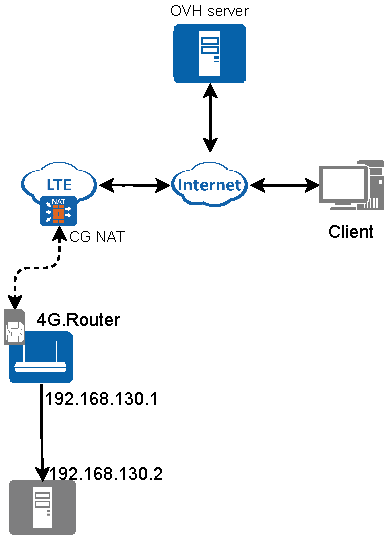
\includegraphics[width=0.44\linewidth]{immagini/diag2-host_real}
    }
    \begin{subfigure}{0.44\linewidth}
        \centering
        \usebox{\myimage}
        \caption{Diagramma di stato degli host domotici}
        \label{fig:diag2-host}
    \end{subfigure}
    \hfill
    \begin{subfigure}{0.53\linewidth}
        \centering
        \raisebox{\dimexpr.5\ht\myimage-.6\height\relax}{
            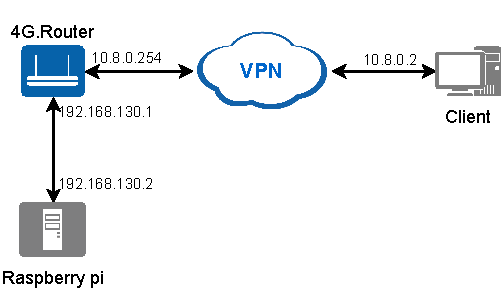
\includegraphics[width=1\linewidth]{immagini/diag2-host_virtual}
        }
        \caption{Diagramma di stato degli host domotici}
        \label{fig:diag2-host1}
    \end{subfigure}
\end{figure}

\section{Configurazione del firewall nel \textit{Router}}

Per rendere possibile la comunicazione tra la rete \it{lan} del \it{Router} e la VPN e' necessario configurare opportunamente il firewall.

Cio' viene fatto direttamente da luci, nella sezione firewall si avranno preconfigurate 2 zone, lan e wan, come si vede figura \ref{fig:luci-firewall-init}.

\begin{figure}[H]
    \centering
    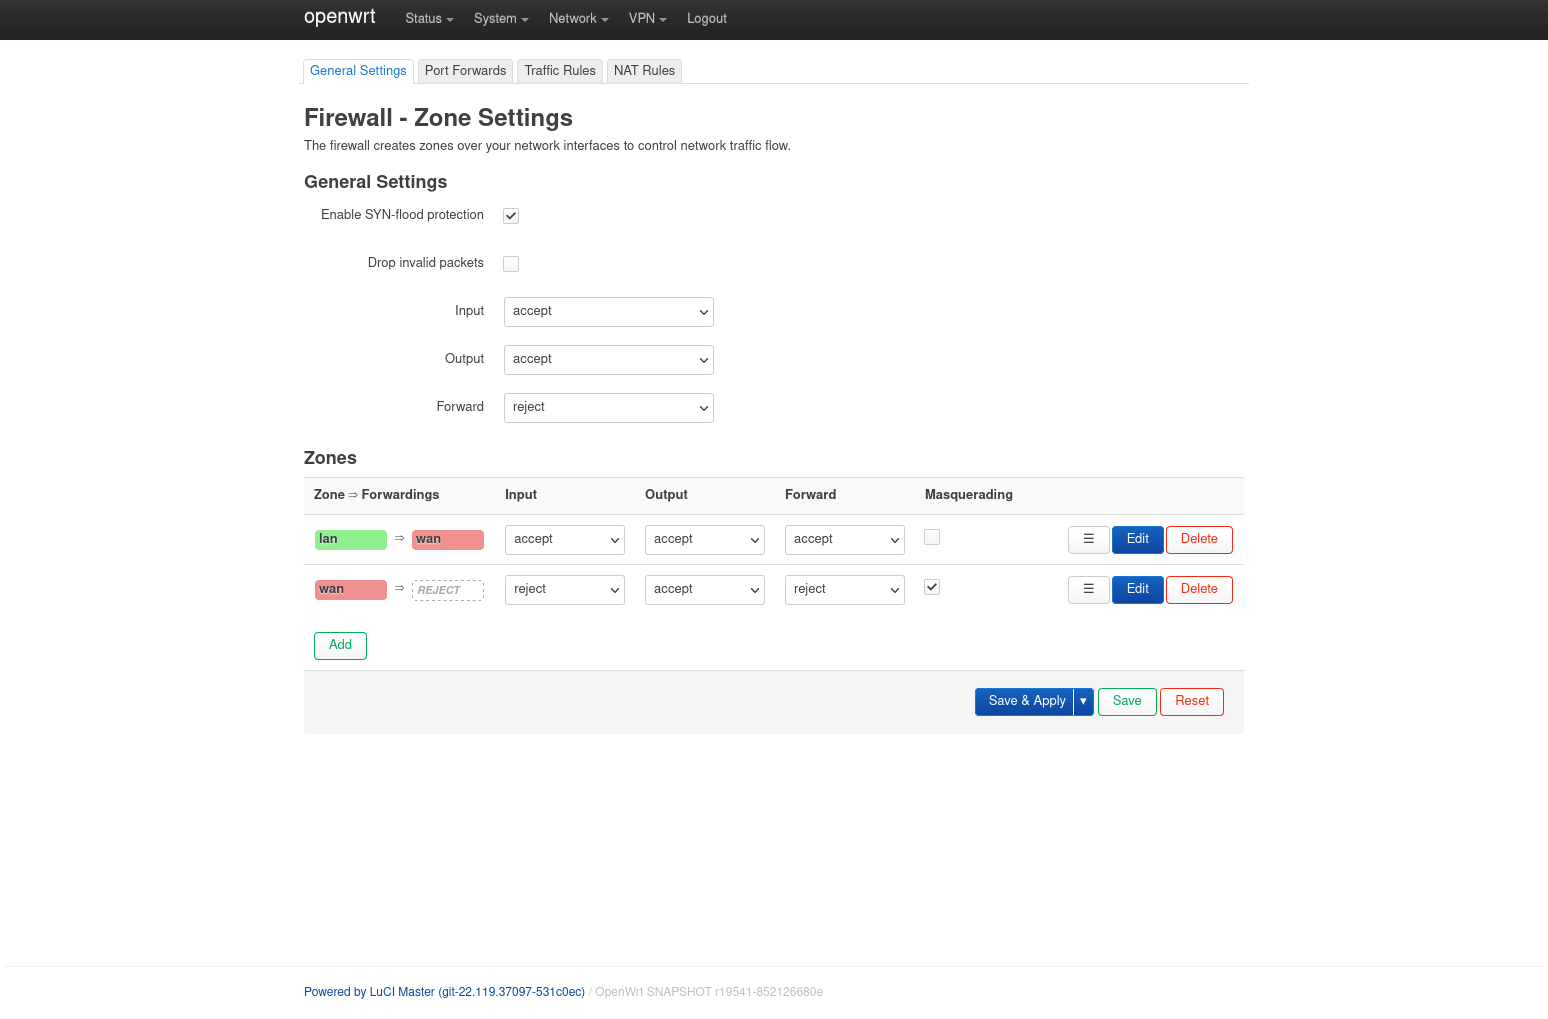
\includegraphics[width=0.8\linewidth]{immagini/LuCI_firewall_init}
    \caption{Configurazione iniziale del firewall}
    \label{fig:luci-firewall-init}
\end{figure}

Si deve quindi aggiungere una nuova zona, chiamata vpn, con le seguenti opzioni:
\begin{itemize}
    \item Policy di forward: accept
    \item Forward consentito verso la zona lan
    \item Forward consentito dalla zona lan
\end{itemize}

\begin{figure}[H]
    \centering
    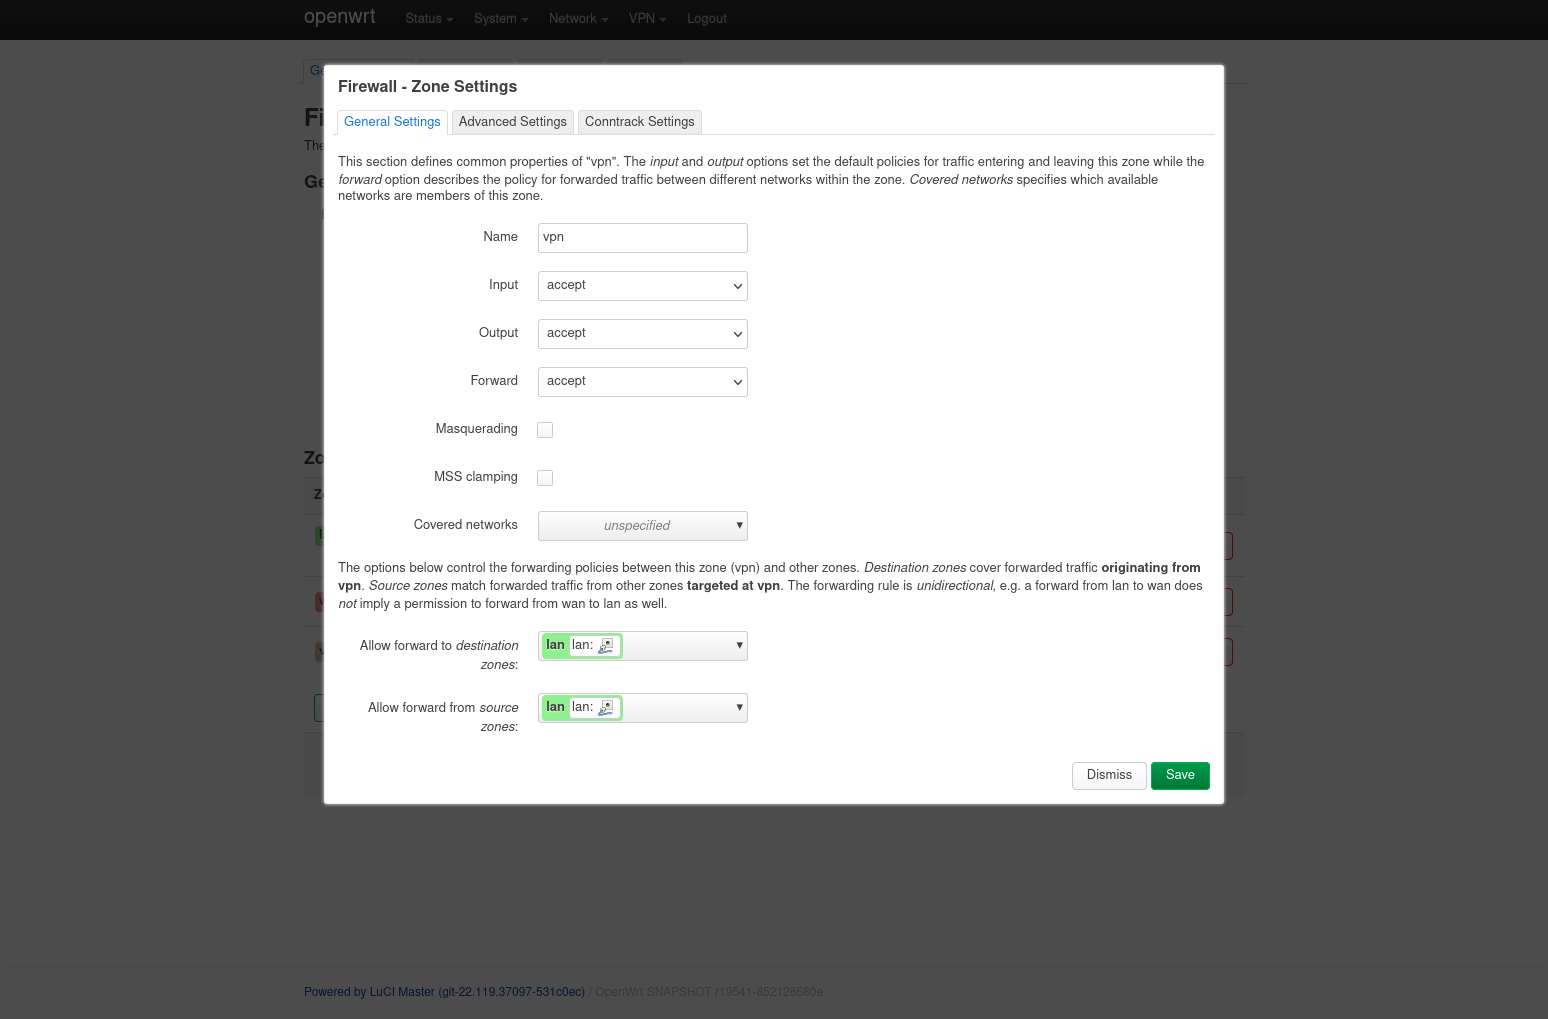
\includegraphics[width=0.8\linewidth]{immagini/LuCI_firewall_vpn}
    \caption{Configurazione del firewall}
    \label{fig:luci-firewall-vpn}
\end{figure}

Dopo aver salvato, la pagina del firewall sara':

\begin{figure}[H]
    \centering
    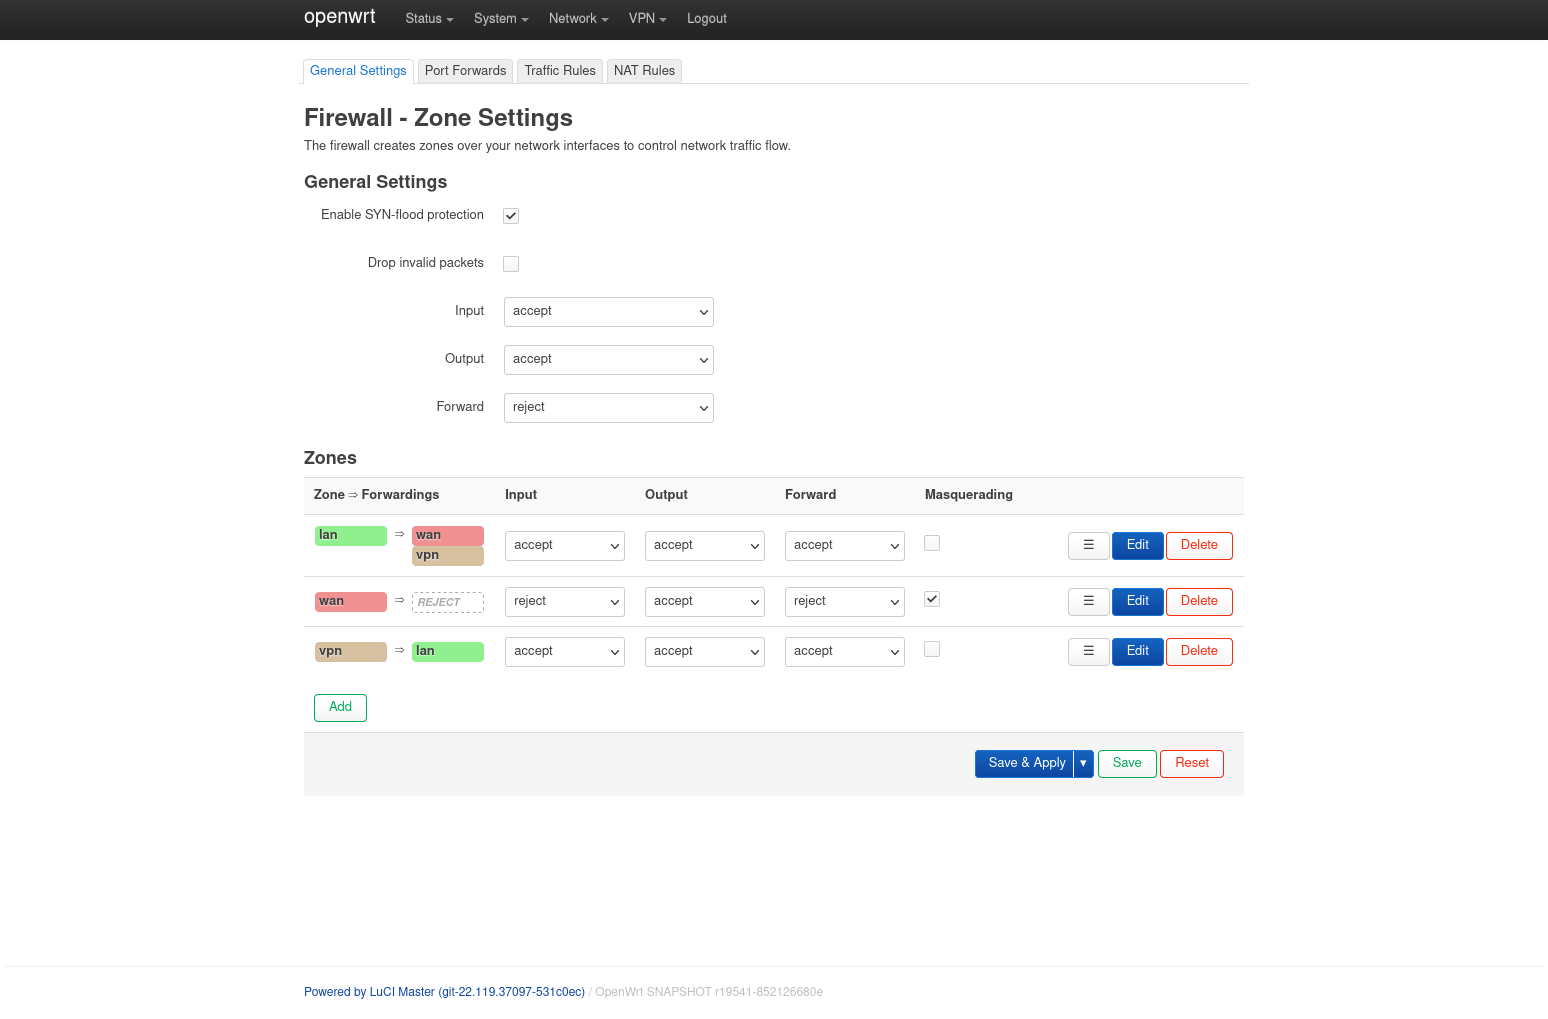
\includegraphics[width=0.8\linewidth]{immagini/LuCI_firewall_end}
    \caption{Configurazione finale del firewall}
    \label{fig:luci-firewall-end}
\end{figure}